\section{Hello, world! | 你好,世界!}
\label{sec:begin:hello-world}

\say[Brian Kernighan]{0.42}{
    \emph{Hello World} is a very simple program,
    but it contains all the basic elements of computer science.
}

\subsection{What is \emph{Programming}? | 什么是编程?}
\label{subsec:begin:hello-world:what-is-programming}

关于 ``什么是编程?'',到网上去搜索这个问题会可以看到各式各样的答案,
但是这么多答案对于新手而言,未免太过繁杂,更别说还有些答案间可能的矛盾,
增加了理解的成本,吓跑了许多 ``初窥门径'' 的人。

对于这个问题,我的答案非常简单:

\begin{quotation}
    \large\textit{
        编程就是通过编程语言让计算机帮我们完成 ``\emph{计算}''}
\end{quotation}

这里的 ``计算'' 指的不仅仅是数学上的运算,还包括了各种各样的数据处理与生成。

\subsection{What is \Py? | 什么是 \Py?}
\label{subsec:begin:hello-world:what-is-python}

那么 \Py 在这里是什么作用呢?其实 \Py 就是人与计算机间的一个翻译官!

电脑其实是无法直接听懂我们说话的,我们想要计算机帮我们做事,
就必须要用某种方式让电脑听懂我们的要求,这个方式就是编程,
其中的媒介就是编程语言,而 \Py 正是一门编程语言。

关于 \Py 的正式介绍如下:

\say[\Py{} Docs]{0.8}{
    \Py 是一种解释型、交互式、面向对象的编程语言。
    它包含了模块、异常、动态类型、高层级动态数据类型以及类等特性。
    在面向对象编程以外它还支持多种编程范式,例如过程式和函数式编程等。
    \Py 结合了超强的功能和极清晰的语法。
    它带有许多系统调用和库以及多种窗口系统的接口,并且能用 C 或 C++ 来进行扩展。
    它还可用作需要可编程接口的应用程序的扩展语言。
    最后,\Py 非常易于移植:它可以在包括 Linux 和 macOS 在内的许多 Unix 变种以及 Windows 上运行
}

总之,\Py 是一门非常厉害的编程语言,我们可以用 \Py 做非常多的事情。

\subsection{first code | 第一行代码}
\label{subsec:begin:hello-world:first-code}

我们学习还是要脚踏实地,所以我们的第一个 \Py 程序 --- 按照传统 --- 就是 \emph{Hello World}。

\begin{minted}{python}
print("Hello, world")
\end{minted}

对于这个程序,我们可以使用一个任意一个文本编辑器创建一个文本,要注意文件的后缀要是 \textcolor{red}{\mintinline{text}{.py}},
然后在其中输入这些内容后保存,然后执行 \verb|python3 path/to/file| 就好。

\begin{figure}[H]
    \centering
    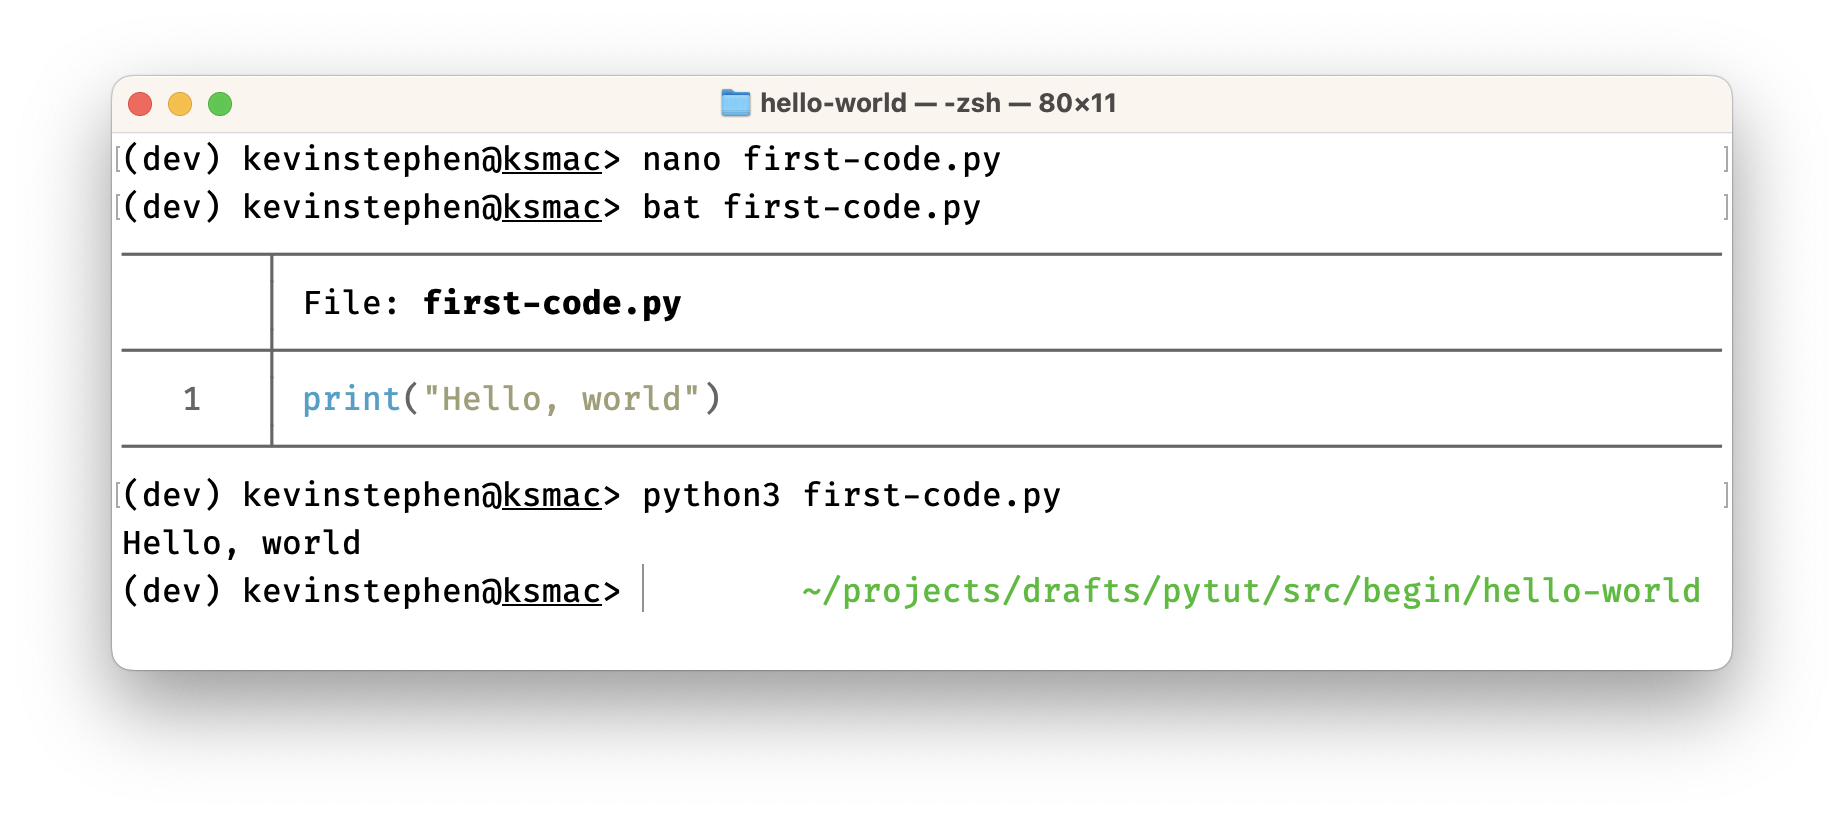
\includegraphics[width=0.8\textwidth]{pics/begin-hello-world-first-code-01.png}
    \caption{使用文本模式}
    \label{fig:begin:hello-world:first-code:01}
\end{figure}

亦或者可以打开终端程序输入 \verb|python3| 或者 \verb|ipython|,
然后输入内容。对于后一种方法,我们一输入内容,就可以看到 ``输出'',
这种就被称为 \emph{REPL},全称是 ``\emph{read evaluate print loop}'',
也就是所谓的 ``交互模式'',对应前一种创建一个文本的方式就称为 ``文本模式''。

\begin{figure}[H]
    \centering
    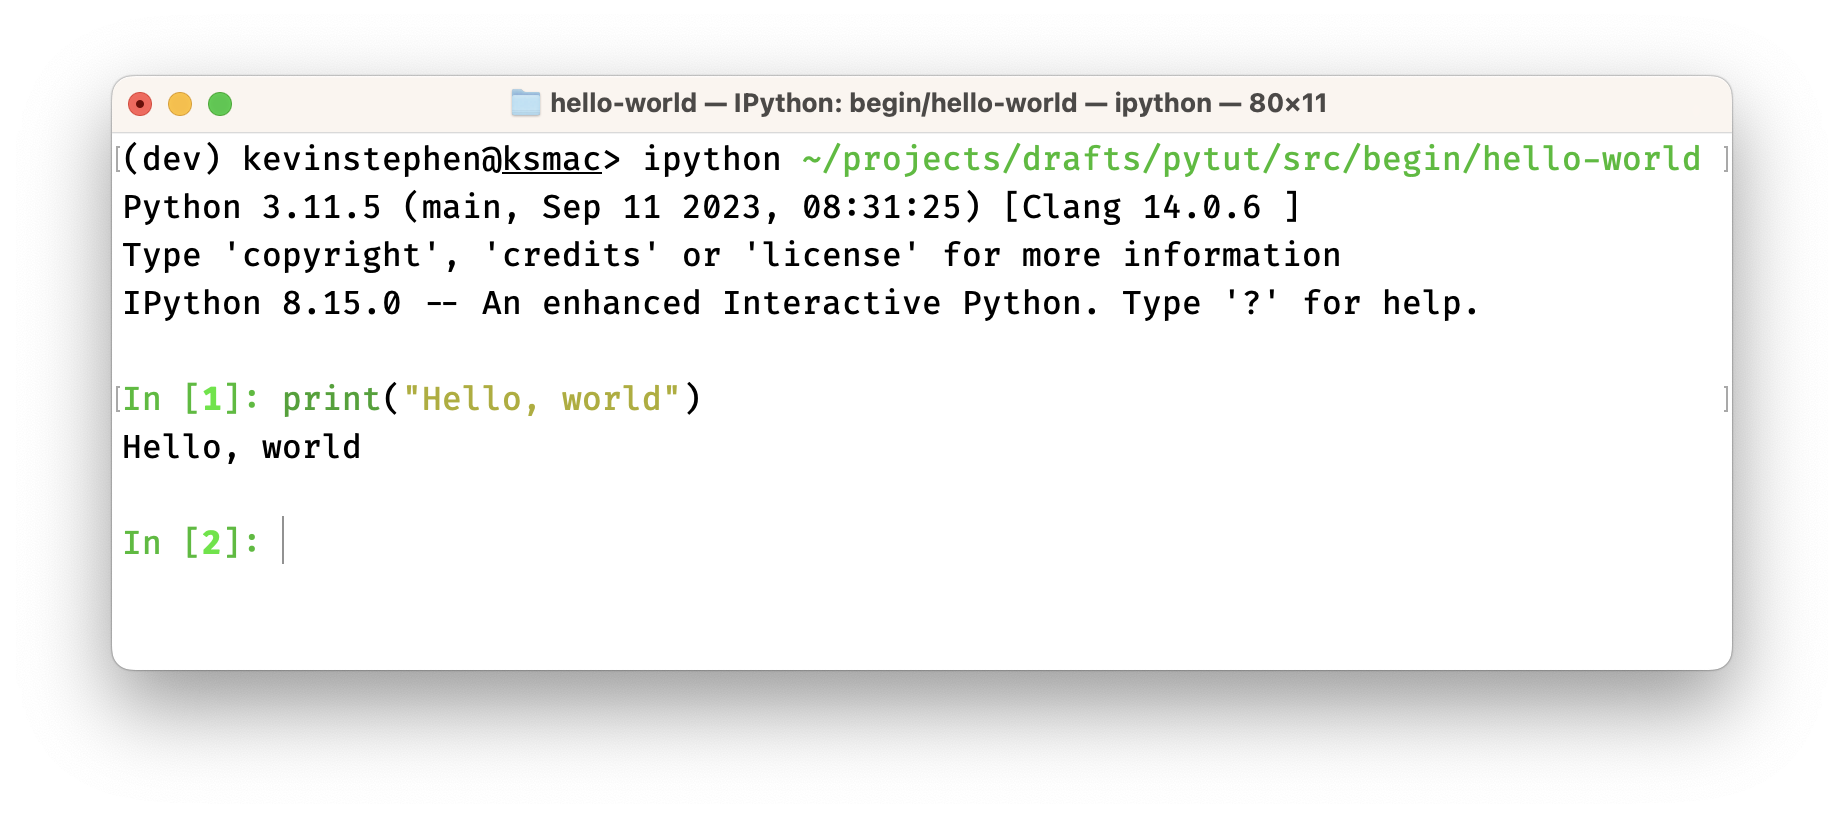
\includegraphics[width=0.8\textwidth]{pics/begin-hello-world-first-code-02.png}
    \caption{使用交互模式}
    \label{fig:begin:hello-world:first-code:02}
\end{figure}
